
\section{Алгоритм (Retriever)}
\label{sec:retriever}

В данной статье основной фокус представлен на то, как можно улучшить уже существующий (пред-обученный) компонент поиска $R$ \eqref{eq:retriever}.
Получив на вход коллекцию из $|D|=N$ документов (параграфов), задача поиска $R$ проиндексировать эти данные в непрерывное метрическое пространство, например, Евклидово - $\Re^n$, 
таким образом, чтобы при входящем запросе $q_i$ выдавать $top_k$ ближайших $top_k\leq 20$ параграфов, подходящих по смыслу.


\subsection{Метрическое пространство}
При работе поисковой системы, на вопрос $q_i$ сопоставляется нейронной моделью $n$-мерный вектор $\vec{v}_i$.
Далее происходит поиск ближайшего векторов, используя алгоритм ближайшего соседа \textit{HNSW} \cite{enwiki:hsnw}. Несмотря на большое разнообразие метрик, в данной работе используется простое скалярное произведение.

\begin{align}
    S(\vec{h_i}, \vec{h_j})=F_{\omega}(q_i) \cdot F_{\omega}(d_j)
    \label{eq:cosine-measure}
\end{align}
% uses a dense encoder $E_P(\cdot)$ which maps any text passage to a $d$-dimensional real-valued vectors and builds an index for all the $M$ passages that we will use for retrieval.
% At run-time, \model/ applies a different encoder $E_Q(\cdot)$ that maps the input question to a $d$-dimensional vector, and retrieves $k$ passages
% of which vectors are the closest to the question vector. We define the similarity between the question and the passage using the dot product of their vectors:
% \begin{align}
%     \mathrm{sim}(q, p) = E_Q(q)^{\intercal} E_P(p).
%     \label{eq:sim}
% \end{align}
% Although more expressive model forms for measuring the similarity between a question and a passage do exist, such as networks consisting of multiple layers of cross attentions, the similarity function needs to be decomposable so that the representations of the collection of passages can be pre-computed.
% Most decomposable similarity functions are some transformations of Euclidean distance (L2). For instance, cosine is equivalent to inner product for unit vectors and the Mahalanobis distance is equivalent to L2 distance in a transformed space.
% Inner product search has been widely used and studied, as well as its connection to cosine similarity and L2 distance~\cite{mussmann2016learning,ram2012maximum}.
% As our ablation study finds other similarity functions perform comparably (Section~\ref{sec:sim_loss}; Appendix~\ref{sec:alt-sim}), we thus choose the simpler inner product function and improve the dense passage retriever by learning better encoders.

\paragraph{Векторные модели отображения (Encoders)}
Реализация нейронного поиска может быть реализована любой нейросетью, но в данной статье выбрано семейство моделей 
\textit{E5} \cite{e5} по двум причинам. Во-первых - они мультиязычны, что необходимо для набора данных $D_u$, т.к. он содержит как англоязычные, так и русскоязычные параграфы (и вопросы к ним соответственно).
Во-вторых, семейство моделей \textit{E5} является SOTA на задаче поиска ``\textit{Semantic Textual Similarity}'' согласно бенчмаркам ``\textit{MTEB}'' \cite{mteb} и ``\textit{RuMTEB}'' \cite{rumteb}.
В третьих, модели \textit{E5} были дополнительно пред-обучены ассиметрично, путем добавления двух разных префиксов к запросам и параграфам. А именно, для запроса использовался используется
$p_{q}=\text{query:}$, а для параграфа, который добавляется в индекс - $p_{d}=\text{passage:}$.

Таким образом, как для параграфов $d_j$, так и для запросов $q_i$, используется ассиметричная модель поиска \textit{E5} (``Small'', ``Base'', ``Large'') с модификацией префикса, согласно предобучению самой модели \cite{e5}.
\begin{align}
    \vec{h}_j&=F(d_j) = F_{\omega}(p_d + d_j) \\
    \vec{h}_i&=F(q_i) = F_{\omega}(p_q + q_i)
    \label{eq:e5}
\end{align}

\paragraph{Поиск ближайшего соседа (ANN)}
Во время работы всей системы, используется сопоставление векторной моделью поиска $F_{\omega}$ \eqref{eq:e5} запроса $q_i$ и, по полученному вектору $\vec{h}_i$ производится 
поиск по индексу, в который были вложены вектора параграфов этой же самой моделью \eqref{eq:e5}. Для реализации поиска алгоритма ближайшего соседа (ANN) применяется реализация 
\textit{Weaviate} \cite{weaviate} - эффективная реализация поиска через \textit{HNSW} алгоритм \url{enwiki:hsnw}, позволяющий индексировать 
данные миллиардных порядков $|D|\ge 10^8$. Фактически, получая на вход запрос $q_i$, через нейронную модель производится вектор $\vec{h}_i$ и, 
среди всех векторов индекса ищется $top_k$ ближайших \eqref{eq:cosine-measure} в метрическом (скалярном) пространстве $\Re^n$, наиболее близких к $\vec{h}_i$.

\subsection{Алгоритм (pipeline)}\label{sec:algo}
На этапе индексации, получив на вход параграфы $D=\{d_j\}$ происходит извлечение ключевых слов и их объяснений в контексте параграфа $d_j$ \eqref{eq:keywords}.

\begin{align}
    \mathrm{Keywords}(d_j) = \{\{k^j_1, e^j_1\}, \cdots, \{k^j_{\sigma(j)}, e^j_{\sigma(j)}\}\}
    \label{eq:keywords}
\end{align}

Извлечение ключевых слов может быть реализовано разными способами, в данной работе использовалась модель \textbf{GPT4-turbo}, с промптом указанным в \href{https://github.com/atomicai/justatom/blob/86f405cf9c6b5bd5cf484636e4d4dcbd10ec0ca1/justatom/running/prompt.py#L16}{prompts.py}. Далее, 
происходит стандартный процесс сопоставления векторов $\vec{v}_j = F_{\omega}(d_j)$ \eqref{eq:e5} указанной моделью и добавление в ANN индекс, используя \textit{Weaviate} \cite{weaviate}.
Самое интересное происходит во время поиска. Для реализации поиска $top_k$ ближайших параграфов к заданному вопросу $q_i$ сначала, как обычно, 
сопоставляется вектор для запроса $\vec{v}_q=F_{\omega}(q_i)$ и, впоследствии делается поиск $top_p >> top_k$ ближайших соседей. Это позволяет учесть большую часть 
всех семантически близких параграфов и, \underline{уже среди ближайших} $top_p$ выбрать необходимые $top_k$, ранжируя их в соответствии с необходимой полнотой выдачи ключевых слов. Отдельный интерес 
представляет функция ранжирования - $\phi$. 

\begin{align}
    \phi& = \gamma_1 \times \phi_s + \gamma_2 \times \phi_r, \gamma_i \in (0, 1)
    \label{eq:phi-global}
\end{align}

В \eqref{eq:phi-global} представлены две функции $\phi_s$ и $\phi_r$. Первая из них - $\phi_s$ это, фактически семантический результат близости векторов. Вторая - 
$\phi_r$ реализует вклад ``ключевых слов''. Вклад ключевых слов можно реализовать множеством способов, однако среди всех перебранных, наилучшей оказалась следующая реализация $\phi_s$:

\begin{small}
\begin{align}
    \sum_{k^j_s, e^j_s \in K_j \cap q_i} \frac{1.0}{\ln(1 + p_{\xi}(w_i))} \times [\sum_{k^j_s, e^j_s \in K_j} \frac{1.0}{\ln(1 + p_{\xi}(w_i))}]^{-1}
\end{align}
\label{eq:idfrecall}
\end{small}

Ранжирование \eqref{eq:idfrecall} представляет собой численный ответ на вопрос: \textbf{Какую часть важных слов контекста ``покрыл'' запрос?}. Так, рассмотрим пример:
При полном совпадении ключевых слов параграфа $K_j$ и запроса $q_i$ - числитель совпадает со знаменателем и $\phi_s(q_i, K_j)=1.0$. Если же, наоборот, 
общих слов нет вообще, то $\phi_r(q_i, K_j)=0.0$. Рассмотрим следующий пример с $q_i$ и выданным контекстом $d_j$, как показано в 
\ref{fig:sample-hunger-games}. $p_{\xi}(w_i)$ - это частота встречаемости слова в контексте. В 
примере из \ref{fig:sample-hunger-games} $p_{\xi}(w_4)=2$ т.к. слово ``арена'' встречается дважды. Оно также входит в запрос $q_i$, поэтому в итоговой сумме будет учтено и в числителе.
Слова: ``трибуты'' и ``мятеж'' не входят в запрос $q_i$, поэтому их учет будет лишь в знаменателе \eqref{eq:idfrecall}. Посчитаем для этого примера полное значение ранжирования $\phi_r$.
\begin{small}
    \begin{align}
        \Omega_1=\frac{1}{\ln(1 + p_{\xi}(w_1))}\approx 1.4427 \\
        \Omega_2=\frac{1}{\ln(1 + p_{\xi}(w_2))}\approx 1.4427 \\
        \Omega_3=\frac{1}{\ln(1 + p_{\xi}(w_3))}\approx 0.9102\\
        \Omega_4=\frac{1}{\ln(1 + p_{\xi}(w_4))}\approx 0.9102
    \end{align}
    \label{eq:calculation-for-sample}
\end{small}

Таким образом, финальная метрика равна:

\begin{small}
    \begin{align}
        \phi_s(q_i, d_j)=\frac{\Omega_1 + \Omega_4}{\Omega_1+\Omega_2+\Omega_3+\Omega_4}\approx 0.5
    \end{align}
\end{small}

Если же из запроса убрать слово ``арена'', что сделает запрос более расплывчатым, т.к. теперь смысл может быть немного другим, то ранжирование будет меньше и равно примерно $\approx 0.3065$

\begin{figure}[ht]
    \centering
    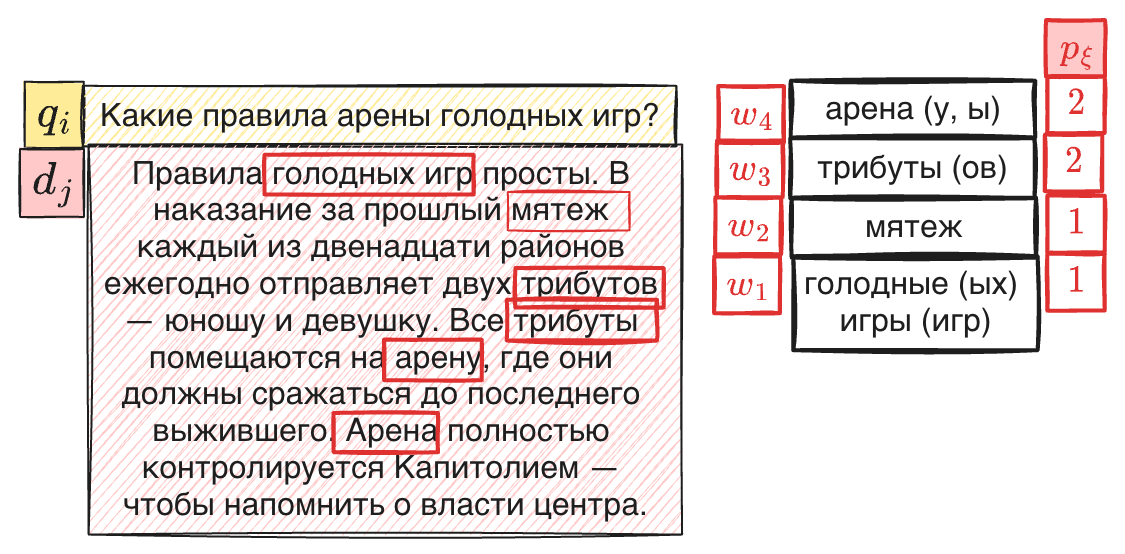
\includegraphics[width=\columnwidth]{figures/sample-hunger-games.png} % Используем ширину одной колонки
    \caption{Демонстрация функции $\phi_s$ на запросе к вселенной  \href{https://w.wiki/DQ\$z}{``Голодные игры''}}
    \label{fig:sample-hunger-games}
\end{figure}


\subsection{Подбор гипер-параметра ($\gamma$)}\label{sec:algo}

Отдельным пунктом рассмотрим, как эффективно подобрать $\gamma$ в \eqref{eq:phi-global}. 
Из-за фиксированного векторного отображения \eqref{eq:e5} фактически уравнение \eqref{eq:phi-global} является функционалом с 
двумя переменными $\gamma_1, \gamma_2$:

\begin{align}
    f(\gamma_1, \gamma_2)& = \gamma_1 \times \phi_s + \gamma_2 \times \phi_r
    \label{eq:gamma-func-forward}
\end{align}

Требуется максимизировать для ``правильных'' пар, т.е. таких $\{q_i, d^+_i\}_{i=1}^{N}$ - требуется оптимально подобрать $\gamma$, 
чтобы максимизировать $f(\gamma_1, \gamma_2) \rightarrow max$. Перегруппировав неизвестные $\gamma_1, \gamma_2$ в \eqref{eq:gamma-func-forward} и сгруппировав его для каждой пары 
$\{q_i, d_i^{+}\}_{i=1}^{N}$, получаем систему пере-определенных линейных уравнений. Такая система, очевидно, не решается алгебраически, а любое ее приближение 
будет крайне ошибочным. В связи с этим, для решения мы используем метод градиентного спуска, до-обучая систему в соответствии с той же функцией ошибки, 
которая использовалась при обучении пред-обученных моделей \textit{E5} \cite{e5}. Таким, образом, для отдельно взятого под-множества (батча) 
$S_i = \{\{q_i, d_i\}, \{q_{i+1}, d_{i+1}\}, \cdots, \{q_{i+|bs| - 1}, d_{i+|bs| - 1}\}\}$, требутеся максимизировать итоговое ранжирование или, что тоже самое, 
минимизировать среднее отклонение по всем батчам $S_i$, для всех $\forall i \in \{1, \cdots, N\}$.
\begin{small}
\begin{align}
   L_{\gamma_1, \gamma_2} = \sum_i-\frac{1}{|S_i|} \sum \log \frac{e^{\phi(q_i, d_i)}}{e^{\phi(q_i, d_i^{+})} + \sum_{j\neq i}e^{\phi(q_i, d_j)}}
    \label{eq:gamma-func}
\end{align}
\end{small}

Как это часто бывает, в некоторых взвешенных функциях, которые суммируют вклад нескольких, отдельно взятых функций, часто 
применяют более простые ранжирования. Так, например, в нашем случая, может показаться, что вполне хватит и одной переменной - $\gamma_1$, вместо двух - 
$\gamma_1, \gamma_2$, выраженная следующим образом: $\gamma_2=1 - \gamma_1$. Однако, как показано ниже на графике, дополнительная связь, не 
помогает максимизировать \eqref{eq:gamma-func-forward}, оставляя большой разрыв между графиками сравнения.

\begin{figure}[ht]
    \centering
    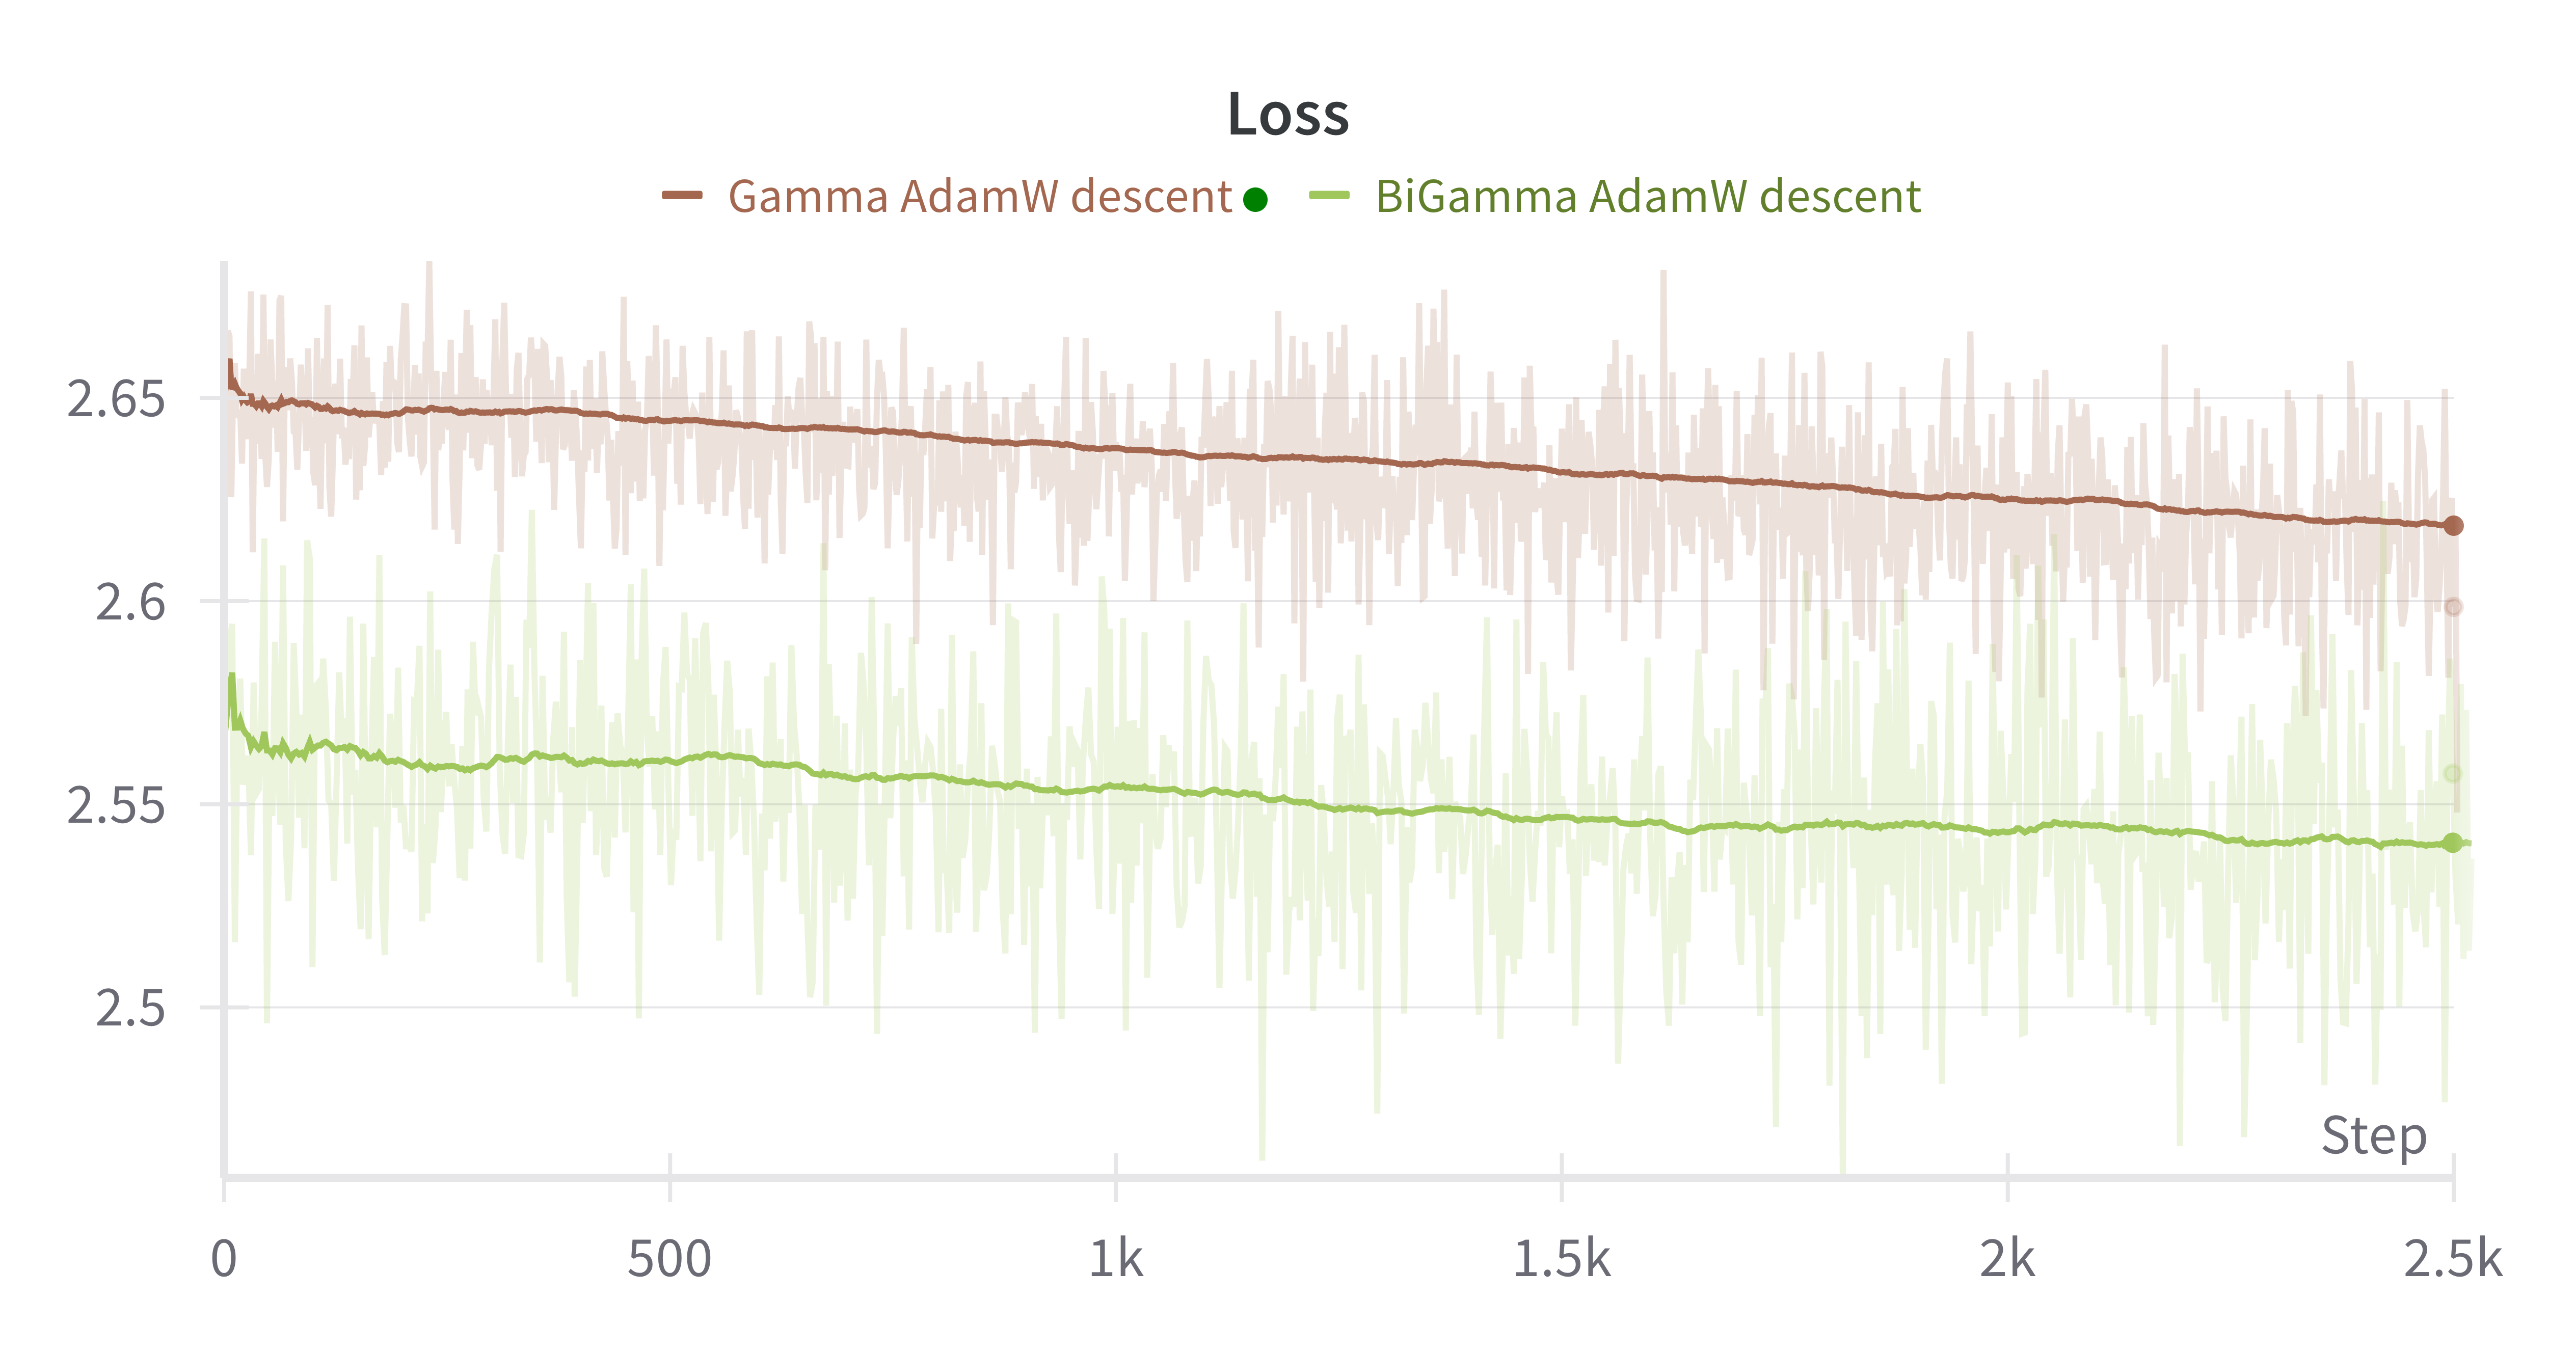
\includegraphics[width=\columnwidth]{figures/Loss-BiGamma-vs-Gamma.png} % Используем ширину одной колонки
    \caption{Сравнение характера функции потерь в \eqref{eq:gamma-func} в разные случаях: $\gamma_1, \gamma_2$ и $\gamma_1 + \gamma_2=1$}
    \label{fig:comparison-gammas}
\end{figure}

\subsection{Сравнительный анализ метрик}

Для функции ранжирования, вполне мог бы подойти и сам текст параграфа. Действительно, код и оставшаяся часть алгоритма никак бы не изменились. 
Однако выбор самого текста параграфа влечет за собой некоторые изъяны, и как показано на графике ниже, аномальные всплески сильно ``ухудшают'' общую метрику, 
приоритезируя выдачу по ключевым словам. Так, например, для набора данных $D_u$ показано сравнения $\phi_r$ на контексте документа и его ключевых словах:

\begin{figure}[ht]
    \centering
    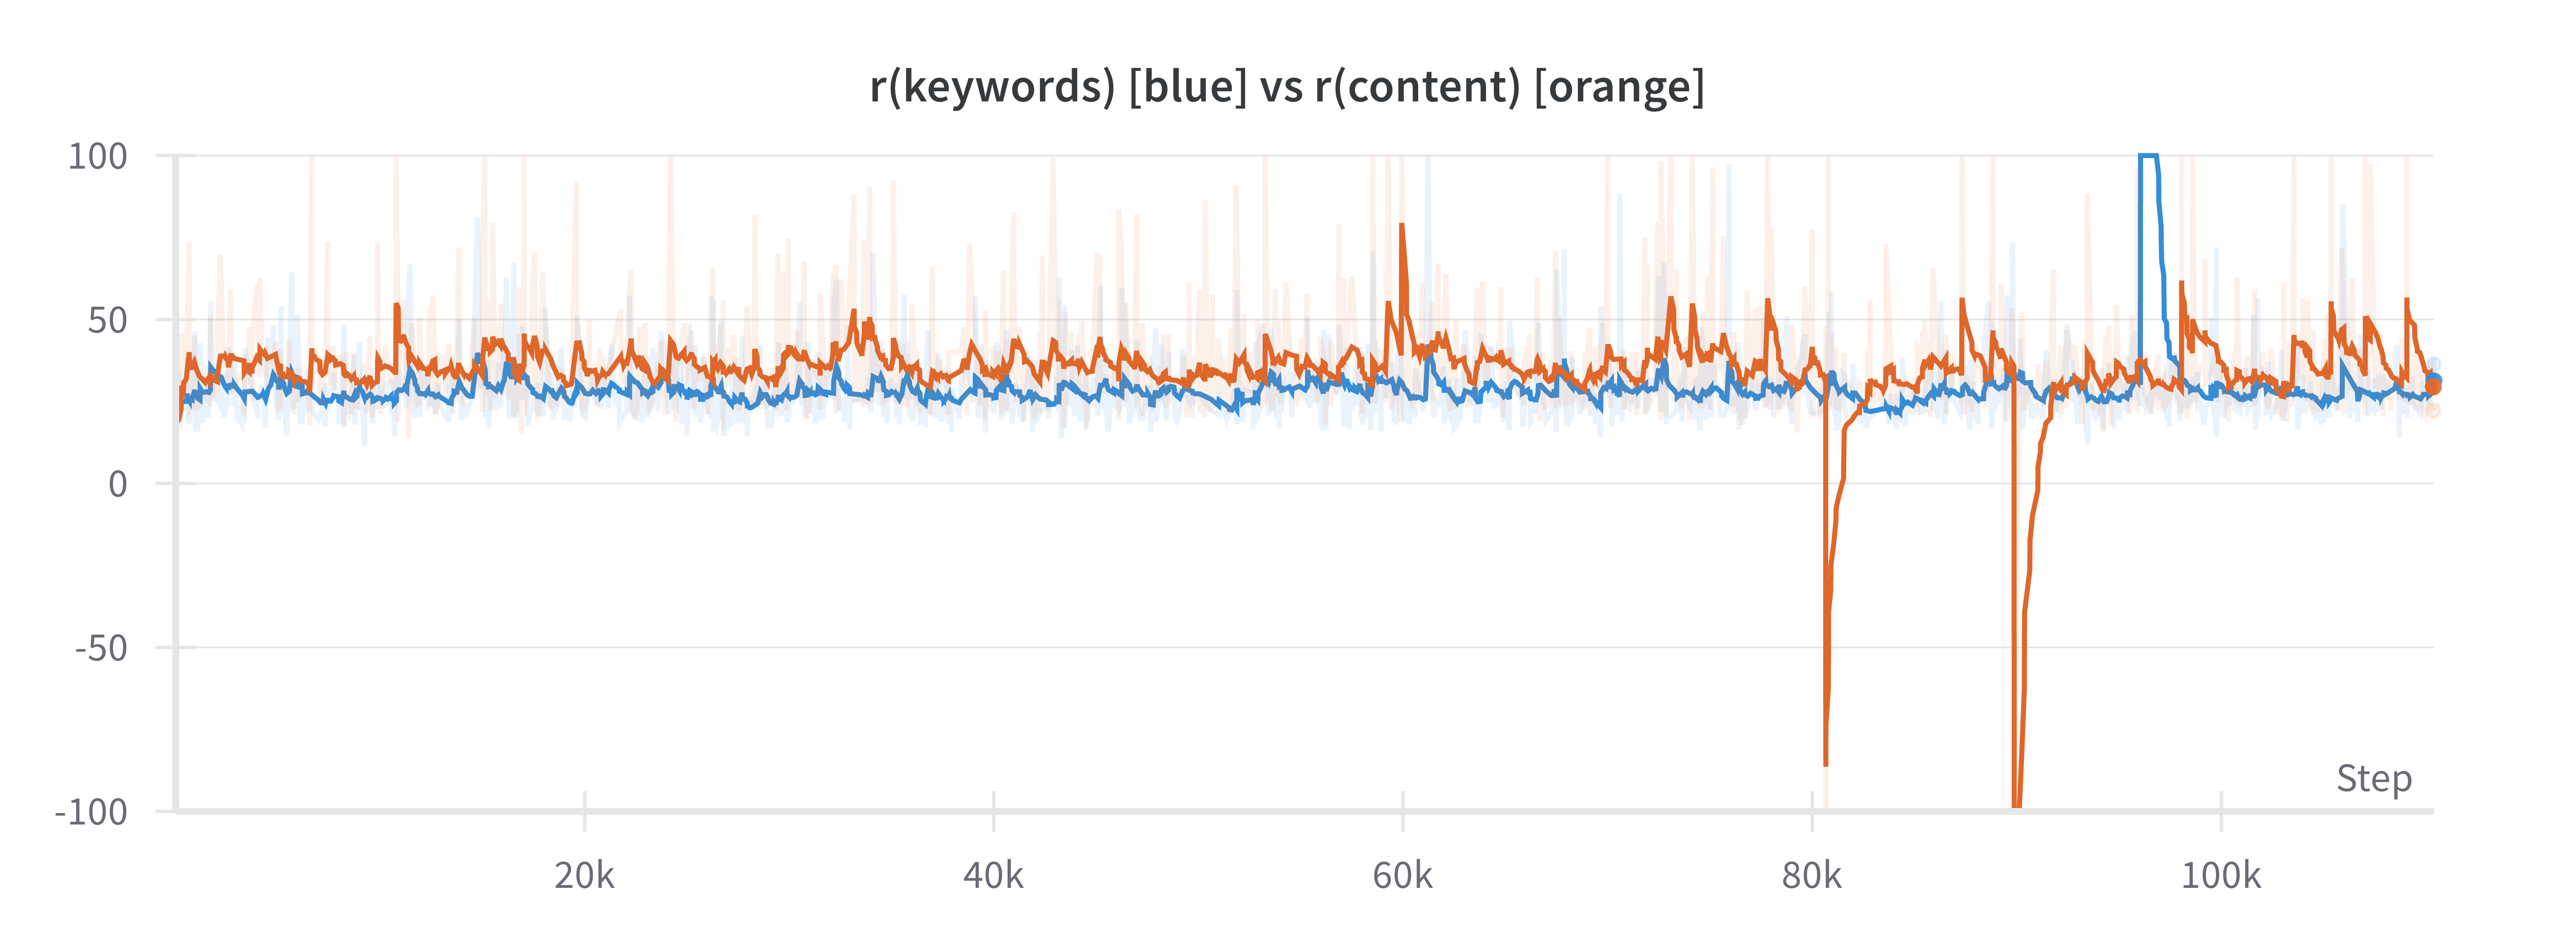
\includegraphics[width=\columnwidth]{figures/idf-recall-content-vs-keywords.png} % Используем ширину одной колонки
    \caption{Сравнение ранжирующей функции $\phi_r$ на примере данных $D_u$}
    \label{fig:comparison-phir-content-vs-keywords}
\end{figure}

Подытоживая вышесказанное, весь алгоритм, в таком случае, визуально представлен ниже:

\begin{figure}[ht]
    \centering
    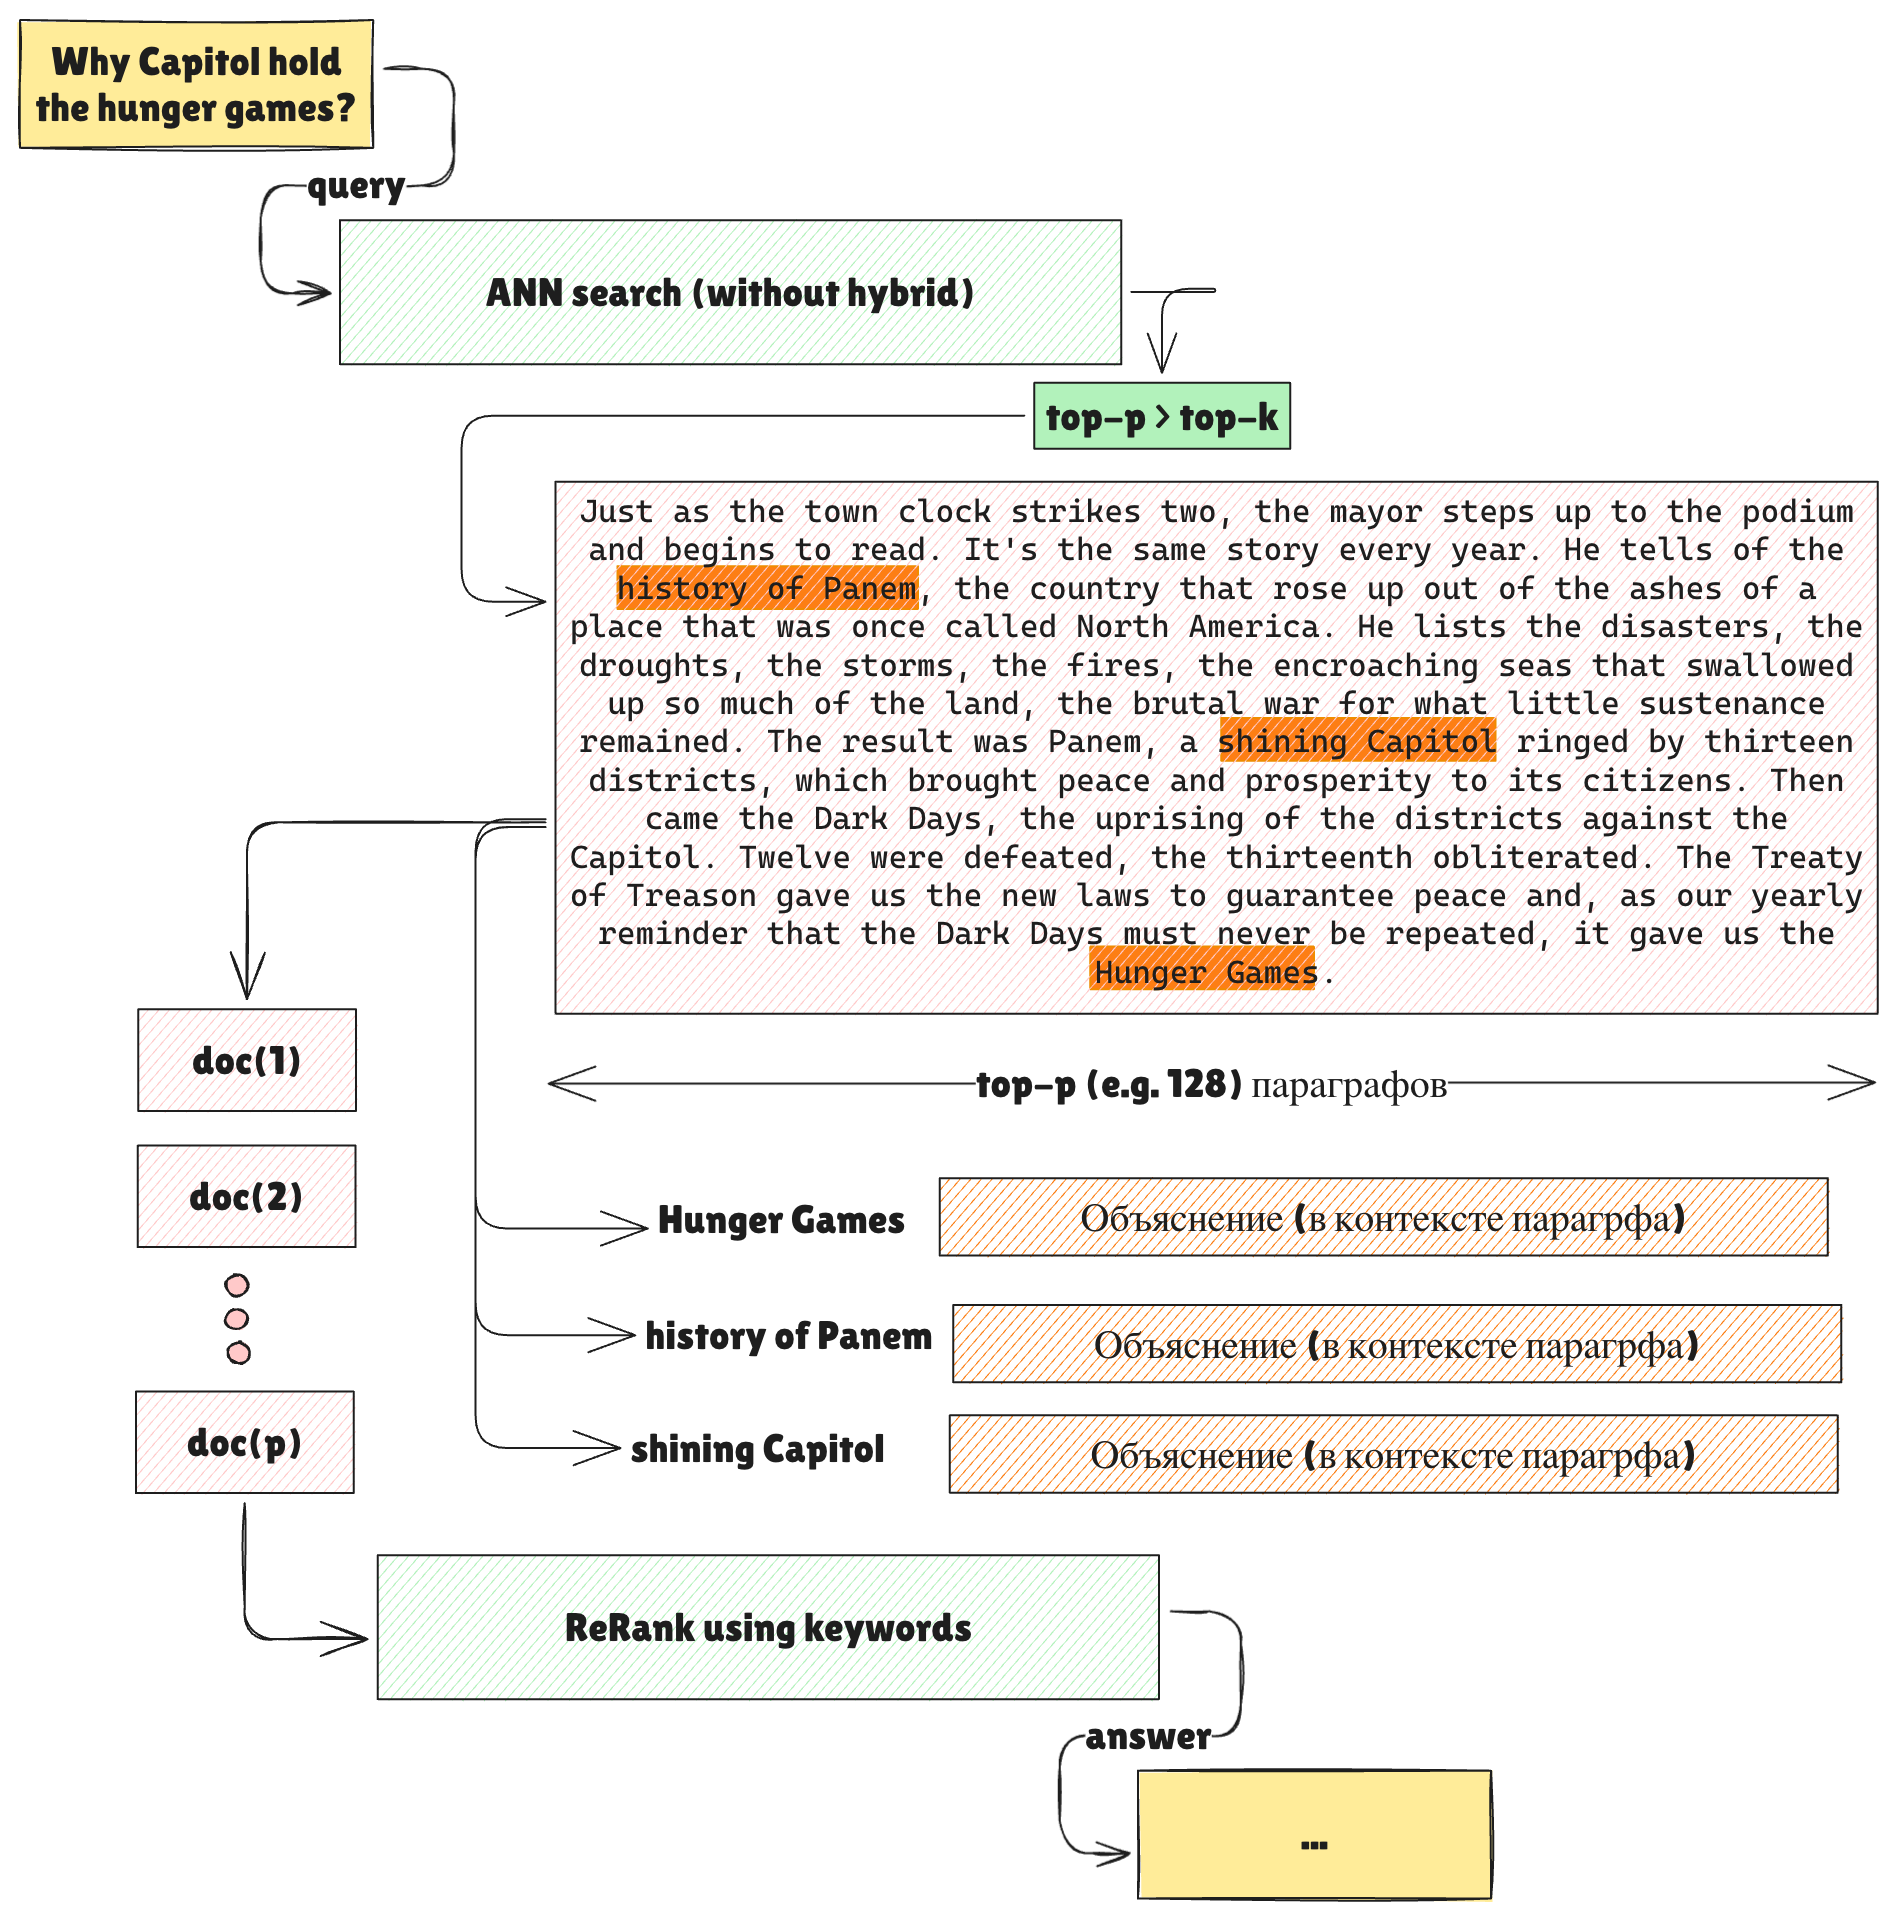
\includegraphics[width=\columnwidth]{figures/top-k-top-p.png} % Используем ширину одной колонки
    \caption{Визуальная демонстрация выбора $top_k \leq top_p$ среди $top_p$ ближайших параграфов}
    \label{fig:comparison-phir-content-vs-keywords}
\end{figure}

Полный псевдо-код описан в \ref{alg:pipeline_for_atomic}.

\begin{figure*}[ht]
% \centering
\makebox[\textwidth]{ % Обеспечивает использование всей ширины страницы
\begin{minipage}{\textwidth}
\begin{algorithm}[H] % Убедитесь, что \caption находится здесь
    \caption{Pipeline for ATOMIC}
    \label{alg:pipeline_for_atomic}
    \begin{algorithmic}[1] % Нумерация строк
    \Procedure{Retrieve}{$Q=\{q_1, q_2, \cdots \}, top_K, top_P$}
        % \State \textbf{$\gamma_1, \gamma_2$} computed $\gets$  \eqref{eq:gamma-func}
        \State \textbf{Compute } $\gamma_1, \gamma_2$ \textbf{ using } \eqref{eq:gamma-func}
        \ForAll{$q_i$ in $Q$}
                    \State \textbf{Maps} $\vec{q_i} \gets F_{\omega}(q_i)$
                    \State \textbf{Search} $D_i \gets R_e({\vec{q_i}})$ 
                    \Comment{Perform ANN search finding $top_P$ closest paragraphs}\\
                    \Comment{Assign them to the variable $D_i = \{d^i_1, \dots, d^i_{top_p}\}$}


                    \ForAll{$d^i_j$ in $D_i$}
                            \State $s^i_j \gets f_{\gamma_1, \gamma_2}(q_i, d^i_j)$
                    \EndFor
                    
                    % --- НОВЫЙ БЛОК: сортируем и берем Top-k ---
                    \State \textbf{Sort} $\hat{D_i} \gets \{d^i_1, \dots, d^i_{top_k}\}$ 
                    \Comment{Let's sort $top_P$ paragraphs returned from $D_i$ according to $s^i_j$}\\
                    \Comment{Select $top_K \leq top_P$ sorted paragraphs from $D_i$}

                    \State \textbf{Yield} $\hat{D_i}$
                    \Comment{Return (yield) the given $top_k$ paragraphs for the $q_i$}
        \EndFor
    \EndProcedure
    \end{algorithmic}
\end{algorithm}
\end{minipage}
}
\end{figure*}
